\section{Miscellaneous Notes}
% the text width in a normal line is 11.80737cm
% To make a TODO note, start a comment with two or more consecutive capital letters.

% Figures are in the gfx folder. They should not have dots in the names
% since that interferes with the crossref function. They should be named
% something like '01-intro.png' where the first two digits are the 
% chapter number and then some simple description of the figure.

% Potential arrangement (for 2nd ed???): 
%		3 Background chapters
%		8 Chapters about ``Traditional'' procedures
%		4 Chapters about Business Analytics, datamining, etc.

% TODO
% Add photo to start of each chapter
% Add whatever graphics I can to each chapter
% Add glossary entries and chapter links 
% Add example research reports

% Start each chapter with a photo and ``Introduction'' paragraph, then the Objectives, then the text, finally, a ``Summary''. 

% Use an ``Objective'' box for objectives and ``Summary'' box for summary. Both boxes are found below. Chapters 1 and 11 have an objectives box at the top and a summary box at the end. Use either as a guide for other chapters.


%******************************************************
\section{3-Line Equation}
%******************************************************
\begin{align}
	\label{03:eq:identity_example}
	1101_2 &= 123 \\
	\nonumber
	&= 123 \\
	\nonumber
	&= 123
\end{align}


\section{Solving an Equation Step-by-step}
\begin{align}
	\label{04:soln:solving_equation_one}
	AB+BC(B+C) && \text{Original Expression} \\
	\nonumber
	AB+BBC+BCC && \text{Distribute BC} \\
	\nonumber
	AB+BC+BC && \text{Idempotence: BB=B and CC=C} \\
	\nonumber
	AB+BC && \text{Idempotence: BC+BC=BC} \\
	\nonumber
	B(A+C) && \text{Factor} \\
\end{align}

%**************************************************************************
\section{Margin Paragraph} 
%**************************************************************************
% Use to create a sidebar paragraph out in the margin
\marginpar{Whatever.}

%**************************************************************************
\section{Footnote Without Marker} 
%**************************************************************************
% Use to create a footnote without a numbering marker
\blfootnote{Whatever.}

%***************************************************************************
\section{Text Box}
%***************************************************************************
% Creates a nice boxed text with a title and main section
\begin{tcolorbox}[colback=blue!5!white,colframe=blue!75!black]
	% Upper half of box: my "title" area
	\textcolor{blue}{\textbf{Interesing Note}}
	% Lower half of the box: the content
	\tcblower
	Whatever.
\end{tcolorbox}

%***************************************************************************
\section{Objectives Box}
% Relies on ``objbox'' in config file
%***************************************************************************
\begin{center}
	\begin{objbox}{Objectives}
		\begin{itemize}
			\setlength{\itemsep}{0pt}
			\setlength{\parskip}{0pt}
			\setlength{\parsep}{0pt}
		
			\item x1.
			\item x2.
			\item x3.
		\end{itemize}
	\end{objbox}
\end{center}

%***************************************************************************
\section{Summary Box}
% Relies on ``tkawybox'' in config file
%***************************************************************************
\begin{center}
	\begin{tkawybox}{Summary}
		\begin{itemize}		
			\item x1.
			\item x2.
			\item x3.
		\end{itemize}
	\end{tkawybox}
\end{center}

%***************************************************************************
\section{Text Table}
%***************************************************************************
\begin{table}[H]
	\centering
	\begin{tabulary}{\linewidth}{LCCCC}
		\hline
		\multicolumn{5}{l}{\textbf{Do you support these propositions?}} \\
		\hline
		Prop & Strongly Support & Support & Do Not Support & Strongly Do Not Support  \\ 
		\hline
		100 & $\bigcirc$ & $\bigcirc$ & $\bigcirc$ & $\bigcirc$ \\ 
		115 & $\bigcirc$ & $\bigcirc$ & $\bigcirc$ & $\bigcirc$ \\ 
		220 & $\bigcirc$ & $\bigcirc$ & $\bigcirc$ & $\bigcirc$ \\ 
		\hline
	\end{tabulary} 
	\caption{My great table.}
	\label{03:tab01}
\end{table}


%***************************************************************************
\section{Text Table v2}
% The 'p{}' values determine the width of each cell
%***************************************************************************
\begin{table}[H]
	\centering
	\definecolor{ltgray}{gray}{0.95} % this is a light gray
	\rowcolors{1}{}{ltgray} % zebra striping background
	\begin{tabularx}{0.95\linewidth}{
			p{0.22\linewidth}
			p{0.22\linewidth}
			p{0.22\linewidth}
			p{0.22\linewidth}}
		\toprule
		\textbf{Party} & \textbf{Clinton} & \textbf{Trump} & \textbf{Other} \\
		\midrule
		Democrats & $ 89\% $ & $ 8\% $ & $ 3\% $ \\
		Republicans & $ 8\% $ & $ 88\% $ & $ 4\% $ \\
		Independents & $ 42\% $ & $ 46\% $ & $ 12\% $ \\
		\bottomrule
	\end{tabularx}
	\caption{2016 Exit Poll.}
	\label{tab06.02}
\end{table}

%***************************************************************************
\section{ToDo}
%***************************************************************************
% Create a ToDo note in the text. This also creates a new clickable TODO
% section in the ``structure'' box on the left side of the page.
%TODO This is a todo note.

%***************************************************************************
\section{Code Snip}
%***************************************************************************
\lstset{ %
  caption={caption},
  label=SL:lst:listing01,
  numbers=left,
  language=Verilog
}
\begin{lstlisting}
  Code here
\end{lstlisting}

%***************************************************************************
\section{Introductory Figure}
%**************************************************************************
% Use this for figures at the top of each chapter

\begin{wrapfigure}{r}{0.4\textwidth}
	\centering
	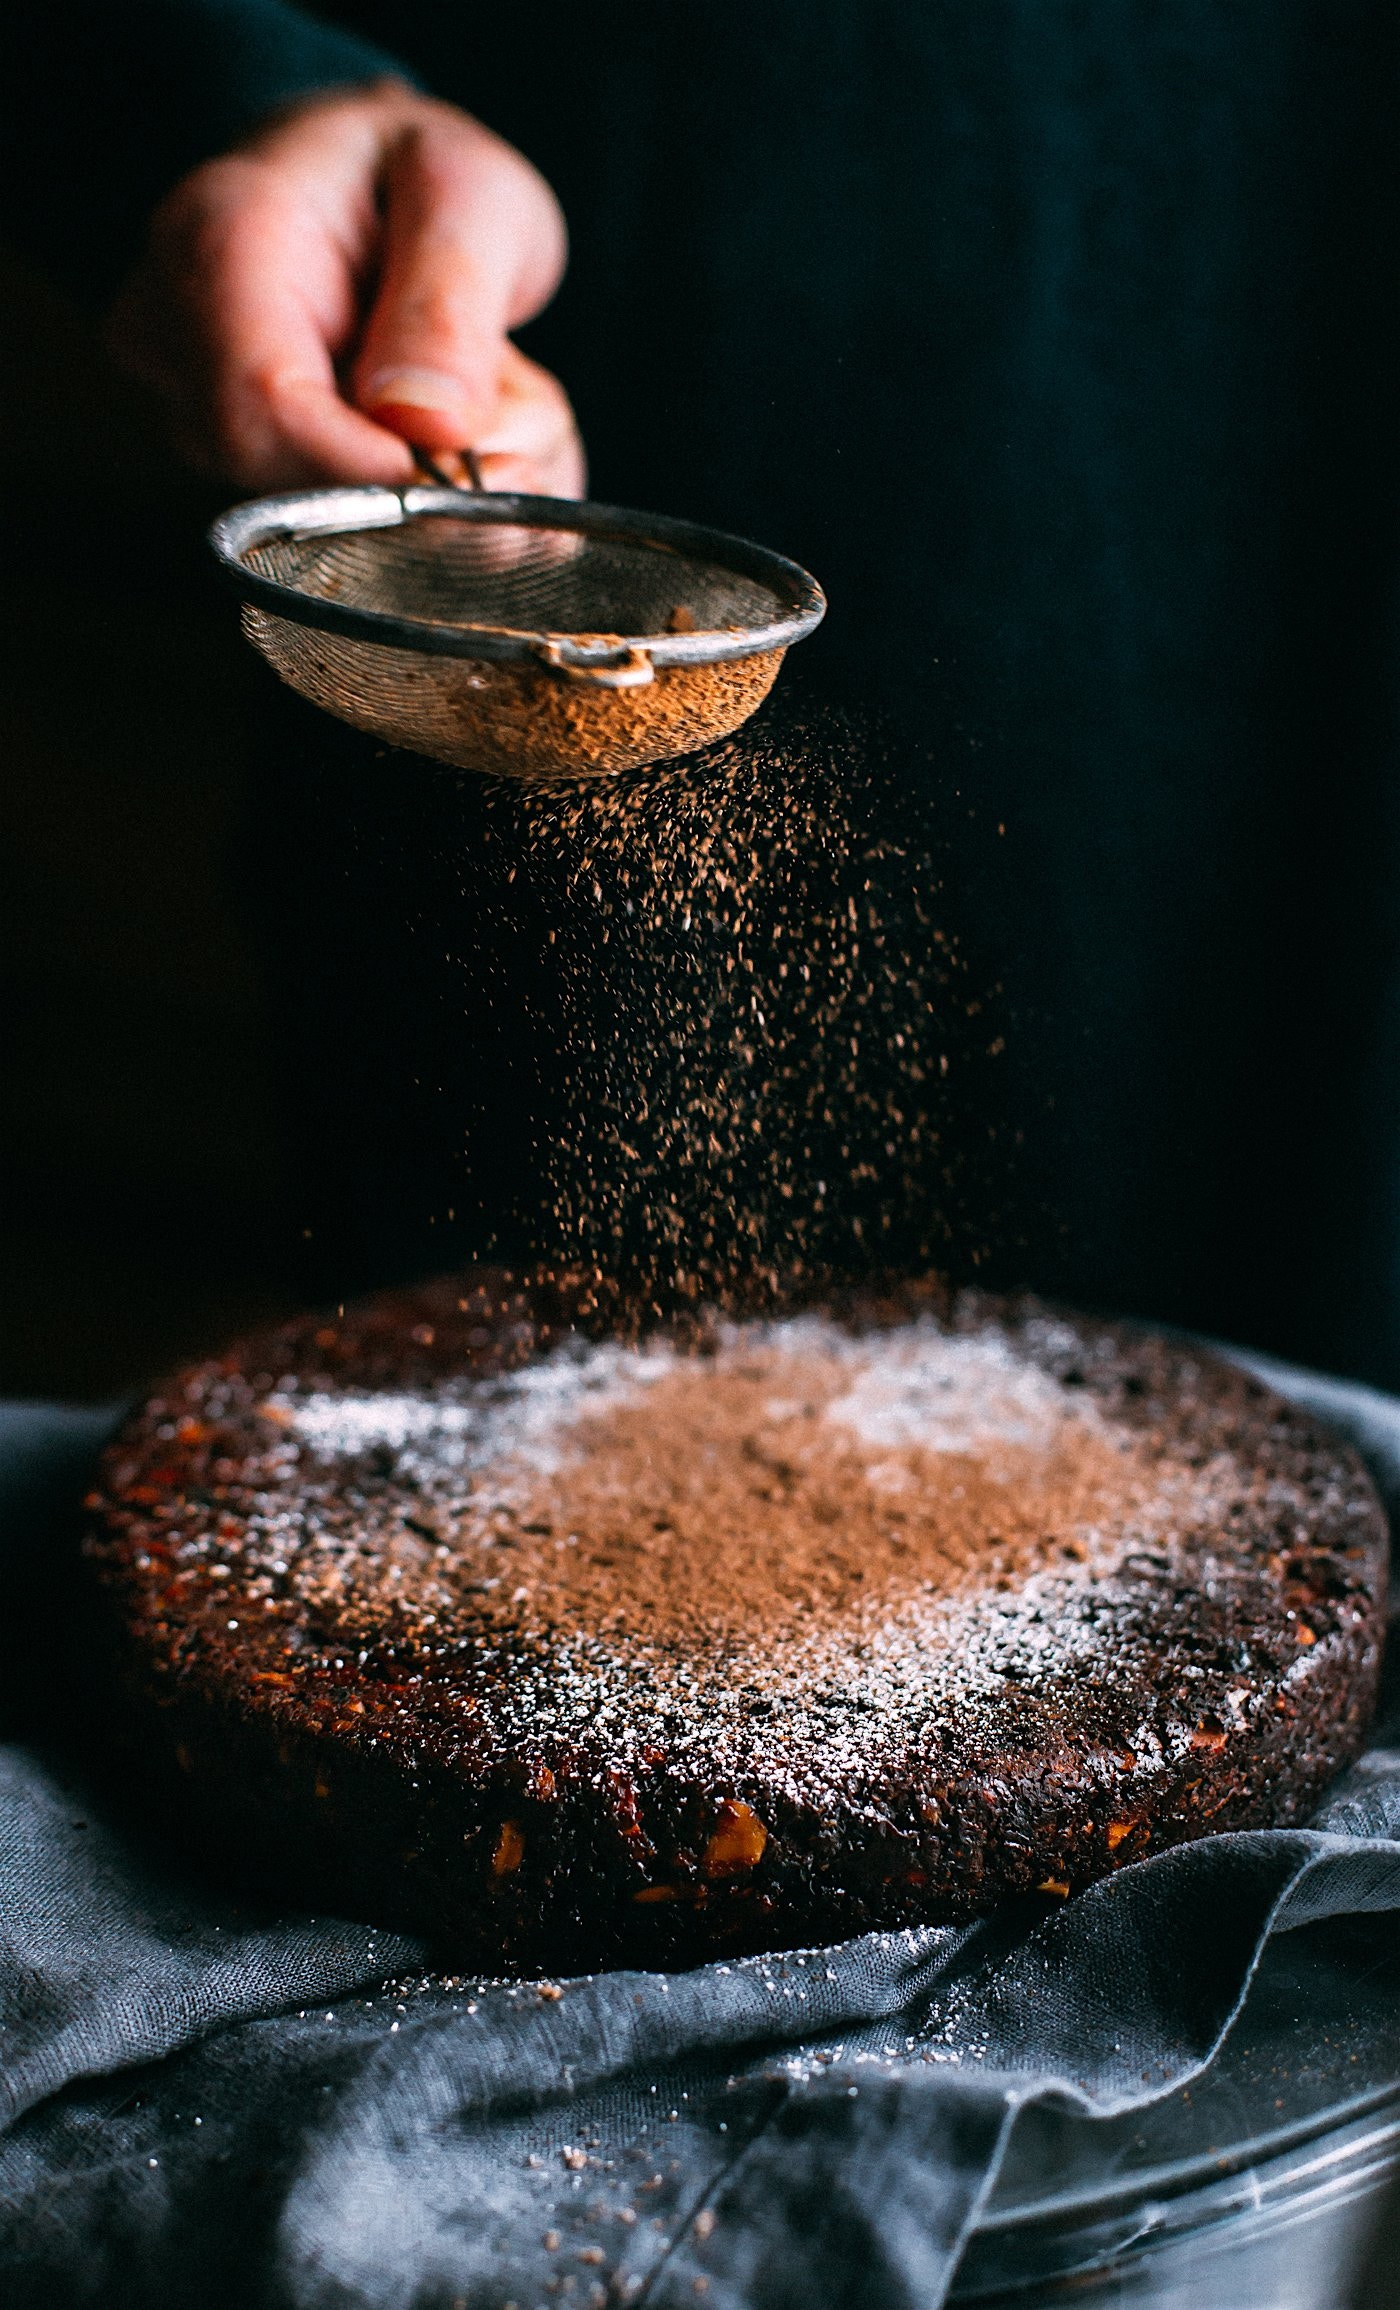
\includegraphics[width=0.4\textwidth]{gfx/05-cake} 
\end{wrapfigure}

First paragraph.\blfootnote{Photo by lindsay Cotter on Unsplash}

%***************************************************************************
\section{Wrap Figure}
%**************************************************************************
\begin{wrapfigure}{O}{0.2\textwidth}
	\caption{} % No text, wraps badly in very narrow space (does print fig number)
	\label{03:fig02} 
	\centering
	
\includegraphics[width=0.2\textwidth]{gfx/99-placeholder} 
\end{wrapfigure}

%***************************************************************************
\section{Regular Figure}
%**************************************************************************
\begin{figure}[H]
	\centering
	
\includegraphics[width=\maxwidth{.95\linewidth}]{gfx/99-placeholder}
	\caption{Caption}
	\label{03:fig03}
\end{figure}

%***************************************************************************
\section{Style Guide}
%**************************************************************************

For menu selections:
Click \textsc{\fbox{Analyze $ \rightarrow $ Descriptive Statistics $ \rightarrow $ Frequencies}}

Labels should be a chapter, colon, verbal desc (all lc with underscores): \label{03:title}
For figures, label should be chapter, colon, ``fig'' and number: \label{03:fig01}

Dates do not include an apostrophe: In the 1960s this happened...

Wrap all numbers in an in-line math block: $ 123 $

